\documentclass{article}
\usepackage{graphicx} % Required for inserting images
\usepackage{multicol} % Allows for multiple columns
\usepackage{float}     % For the H option

\title{\textbf{CS739 Mini-Project 2 Result Summary}}
\author{
    \begin{minipage}[t]{0.45\textwidth}
        \begin{flushleft}
            \textbf{Team Members:} \\
            Tyler Wilson \\ 
            Surendra Parla \\ 
            Sree Kandasamy Gokulrajan \\ 
            Tianyu Huang
        \end{flushleft}
    \end{minipage}
    \hfill
    \begin{minipage}[t]{0.45\textwidth}
        \begin{flushright}
            \textbf{Partner Team:} \\
            Harsha Varthan Chellaiah Ramamoorthy \\ 
            Souvik Roy \\ 
            Wenxuan Tan \\ 
            Zeren Yang
        \end{flushright}
    \end{minipage}
}
\begin{document}

\maketitle
\section{Partner Group's Test Result}
\subsection{Availability Test}
The main purpose of the test is to simulate and test the availability of a distributed key-value storage system when the number of service nodes is gradually reduced, and to observe the changes in the success rate of PUT and GET operations in the process of reducing server instances.\\
At first, we started 100 server nodes, and then used kv739\_die() function to shut down the nodes one by one and observe the changes in the success rate.
\subsubsection{Availability Test Result}
\begin{figure}[H]  
    \centering
    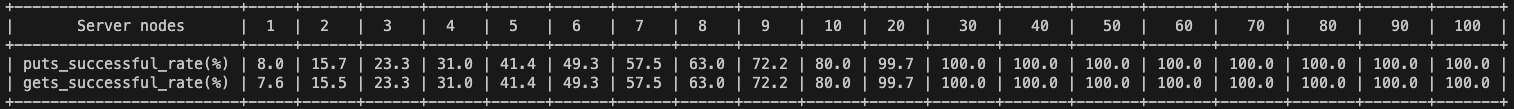
\includegraphics[width=1\textwidth]{ptn_availability_output_table.png}  % Adjust width
    \caption{Availability Result Table}
\end{figure}
\begin{figure}[H]  
    \centering
    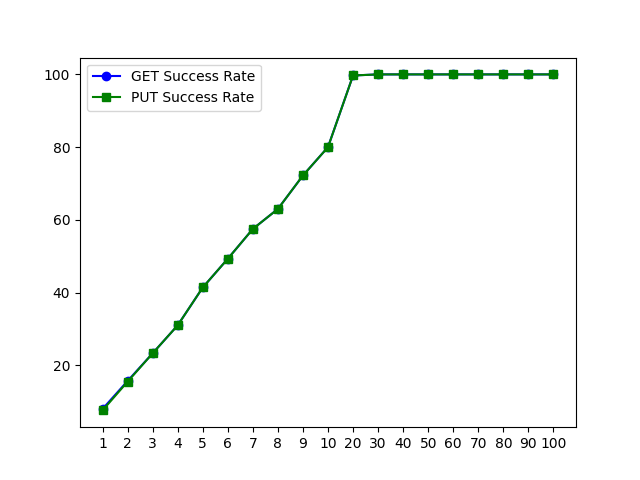
\includegraphics[width=1\textwidth]{ptn_availability_output_plot.png}  % Adjust width
    \caption{Availability Result Graph}
\end{figure}
It can be seen that when the number of server nodes is greater than 20, the success rate is 100\%, when the number below 20, the success rate begin to decline. The minimum number of server nodes that can operate normally is about 16.

\subsection{Consistency Test}
The purpose is to simulate multiple clients accessing the distributed key-value storage system at the same time, perform consistency testing, and record the ratio of successful operations to observe whether the success rate of the system is affected as the number of clients changes.\\
After each client PUTs a key-value pair, it immediately GETs the value and verifies that the value it gets is consistent with the value it PUT. Any inconsistencies (such as GET results that are different from the PUT values) are recorded.

\subsubsection{Consistency Test Result}
\begin{figure}[H]  
    \centering
    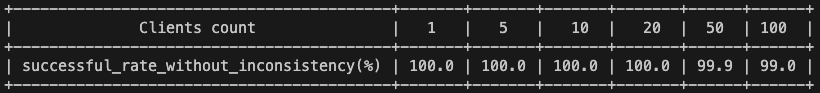
\includegraphics[width=1\textwidth]{ptn_consistency_output_table.png}  % Adjust width
    \caption{Consistency Result Table}
\end{figure}
\begin{figure}[H]  
    \centering
    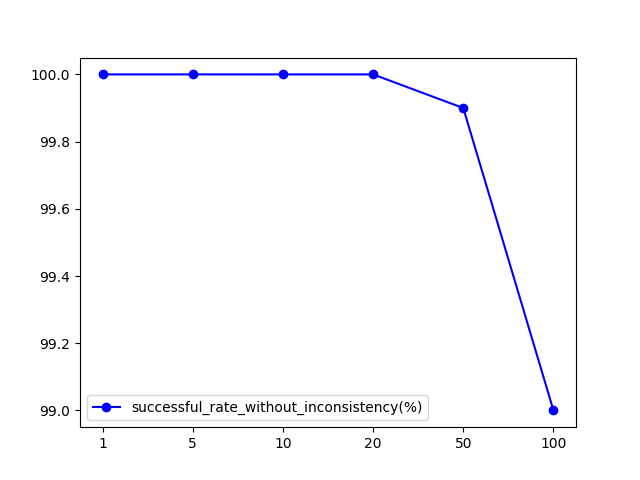
\includegraphics[width=1\textwidth]{ptn_consistency_output_plot.png}  % Adjust width
    \caption{Consistency Result Graph}
\end{figure}

\subsection{Performance Test}
The purpose is to measure the performance of the system, especially latency and throughput, by simulating PUT and GET operations of multiple clients on the distributed key-value storage system. It can also test the performance of the system when a certain proportion of hot keys are frequently accessed. Our results are the average of 10\%, 20\%, and 30\% hot keys.

\subsubsection{Performance Test Result}
\begin{figure}[H]  
    \centering
    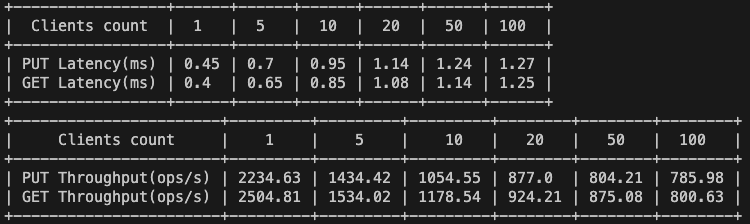
\includegraphics[width=1\textwidth]{ptn_performance_output_table.png}  
    \caption{Performance Result Table}
\end{figure}
\begin{figure}[H]  
    \centering
    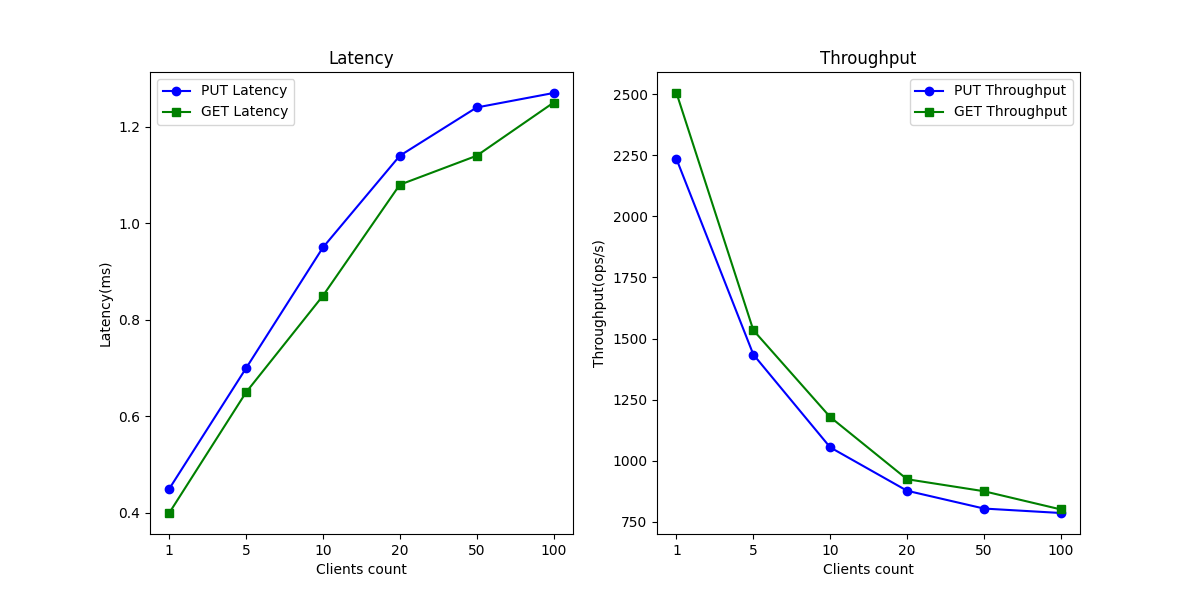
\includegraphics[width=1\textwidth]{ptn_performance_output_plot.png}  
    \caption{Performance Result Graph}
\end{figure}


\end{document}